%% LyX 2.0.1 created this file.  For more info, see http://www.lyx.org/.
%% Do not edit unless you really know what you are doing.
\documentclass[english]{article}
\usepackage[T1]{fontenc}
\usepackage[latin9]{inputenc}
\usepackage{geometry}
\geometry{verbose,tmargin=1in,lmargin=1in,rmargin=1in}
\usepackage{array}
\usepackage{varioref}
\usepackage{float}
\usepackage{multirow}
\usepackage{amstext}
\usepackage{graphicx}
\usepackage{setspace}
\usepackage[authoryear]{natbib}
\doublespacing
\usepackage{nameref}

\makeatletter

%%%%%%%%%%%%%%%%%%%%%%%%%%%%%% LyX specific LaTeX commands.
\DeclareRobustCommand{\greektext}{%
  \fontencoding{LGR}\selectfont\def\encodingdefault{LGR}}
\DeclareRobustCommand{\textgreek}[1]{\leavevmode{\greektext #1}}
\DeclareFontEncoding{LGR}{}{}
\DeclareTextSymbol{\~}{LGR}{126}
%% Because html converters don't know tabularnewline
\providecommand{\tabularnewline}{\\}
%% A simple dot to overcome graphicx limitations
\newcommand{\lyxdot}{.}


%%%%%%%%%%%%%%%%%%%%%%%%%%%%%% User specified LaTeX commands.
\usepackage{multicol} 

\makeatother

\usepackage{babel}
\begin{document}

\title{Morphological Recomposition: An MEEG Study}


\author{Teon Brooks}


\date{September 4, 2012}

\maketitle
\pagebreak{}


\section{Introduction}

From words and to sentences and beyond, language has a fascinating
ability to compose basic units to express new and complex meanings.
Much research has been done in the past thirty years investigating
the mechanisms of word recognition. The understanding how words are
organized and arranged has been a lively and contentious topic within
the field of language research. Morphemes are smallest pairing of
a sound to a meaning wherein the word 'walker' would consist of two
morphemes, 'walk' and '-er'. The field tends to be split over lexical
storage, i.e. whether morphologically complex words, words with more
than morpheme, are stored as solitary units irrespective of internal
structure (list-memory approach, e.g. 'WALKER'), or as stems (basis
for word-formation) and computed with other morphemes (morphemic approach,
e.g. 'WALK' + '-ER').


\subsection{Morphological decomposition}

The field has begun to converge on a morphemic approach to word storage.
\citet{Taft:1975fd} proposed some of the earliest models in lexical
storage of affixed words. Using lexical decision \citep{Meyer:1971uq}
to test the predictions of their model, they proposed that the lexicon
is arranged by word frequency and that stems of derived words are
stored as lexical items. \citet{Marslen-Wilson:1994er} detailed a
more comprehensive model of the mental lexicon in which they claim
that this morphemic organization is semantically constrained. They
found that words with possible morphemic constituents (e.g. depart
+ -ment for department) did not prime their constituent embedded word
(e.g. depart) when their word forms did not contribute to its meaning.

More recent work from \citet{Rastle:2004bh} has propelled the field
to reassess the semantic constraint claim. To test this claim, they
used the lexical property of semantic transparency to determine the
accessibility of possible embedded morphemes. Semantic transparency
describes how well a word's constituent word forms (morphemes) contribute
to its overall meaning. A word is considered semantically transparent
if the constituent meanings contribute to the overall meaning (e.g.
audit + -or for auditor) whereas a word is considered semantically
opaque if there are no meaningful contributions from its possible
word forms (e.g. audit + -tion for audition). To disentangle the effects
of semantic constraints on morpheme segmentation, \citeauthor{Rastle:2004bh}
used a masked priming paradigm to test whether there is an earlier
stage in word recognition that parses word forms on the basis of their
representation in the lexicon, their lexicality. Their premise for
using priming is that when an item is primed, its representation has
been activated leading to faster time in reactivation. Masked priming
allows for this activation to occur at a subliminal level. The results
revealed that there was faster and equal amounts of priming of the
complex word on its constituent word form for both semantically opaque
(e.g. BROTHER-broth) and transparent complex words (e.g. DARKNESS-dark)
but not for simple words with a possible embedded word but no legal
affixes (e.g. BROTHEL-broth). They concluded that these results reflect
a process of morpho-orthographic decomposition where words are parsed
into possible word forms regardless of semantic transparency. Transparent
and opaque complex words alike would go through this process, but
simple words would not be broken down further if the results would
lead to illegal affixes.


\subsection{Morphological composition}

Since these findings there have been more convergent results inline
with these findings, yet little progress has been made in determining
if the word forms parsed in decomposition are recombined for word
recognition or if decomposition is merely an automatic but not necessary
for word recognition. If decomposition feeds into word recognition,
there are some necessary steps in processing, i.e. lexical access
and recomposition, that are needed to reach this stage \citep{Meunier:2007ml}.
Lexical access involves the retrieval of the stored representation
in memory for each of the word forms. Recomposition would involve
the combination of the lexical meanings of the word forms. 

There are proposals for a general binding mechanism for basic composition
proposed by \citet{Bemis:2011zr} that may play a role at the word-level.
The lateral anterior temporal lobe (LATL) and the ventromedial prefrontal
cortex are involved in various semantic combinatorial computations,
i.e. minimal composition and enriched composition, respectively \citep{Bemis:2011zr,Pylkkanen:2007yq}.
In the minimum composition study, \citet{Bemis:2011zr} found that
two composable items, an adjective-noun phrase, revealed more activation
in the LATL and vmPFC than two non-composable items, a random letter
string and word. This was taken as evidence of the most basic of combinatorial
processing. Thus, a model of complex word recognition requires at
least these three stages of process: parsing into basic units (decomposition),
access of their meanings (lexical access) and the recomposition of
these word forms with their meaning \citep{Stockall:2006am,Taft:2004uq}.


\subsection{Time-course of word recognition}

A morphological composition-based model would propose that complex
words would be represented as a construction of its morphemes bound
together in some systematic manner. Research in electrophysiology
and magnetic physiology has begun indexing these stages in visual
word recognition by identifying the time-course of these cognitive
processes. EEG studies first show letter frequency effects starting
around 100ms (N1 on n-gram frequencies: \citealp{Hauk:2006zr}). MEG
studies show activation peaking around 170ms after the presentation
of a stimulus (M170 on morphological decomposition: \citealp{Solomyak:2010vn}).
These decomposition effects appear in the same window but peak somewhat
later in EEG, at around 250ms (N250: \citealp{Morris:2007uq}). Their
source generator has been localized to the left fusiform gyrus \citep{Dehaene:2010qw,Solomyak:2010vn}. 

After these word forms are activated, their lexical access tends to
occur between 250-350ms with activation in the superior temporal gyrus
\citep{Pylkkanen:2003fk}. Although there is little to no research
on how word forms are recomposed, we propose that their recombination
uses the same basic combinatorial areas, specifically LATL and orbitofrontal
cortex, proposed by \citet{Bemis:2011zr}. This combinatorial process
tends to occur from 184 to 255ms in the LATL \citep{Bemis:2011zr}
suggesting that the composition of these word form works in parallel
with their access. Classic models of language comprehension implicated
the pars triangularis (left inferior frontal gyrus (LIFG); Broca's
area) in syntactic construction of words, which may also be a candidate
for a composition area. Although some of these areas interact with
each other to form a general speech processing network, it is still
unclear how well this model extends to the areas involved in visual
word recognition.

\begin{figure}[H]
\begin{centering}
\includegraphics[scale=0.25,bb = 0 0 200 100, draft, type=eps]{/Users/teon/Dropbox/Experiments/NMG/results/rois/R0095_lateral.png}\includegraphics[scale=0.25,bb = 0 0 200 100, draft, type=eps]{/Users/teon/Dropbox/Experiments/NMG/results/rois/R0095_medial.png}\caption{Selected Regions of Interest (Lateral View)}

\par\end{centering}

\caption{Selected Regions of Interest (Sagittal View)}


Five ROIs were defined in this study: Fusiform Gyrus ``orchid purple'',
Temporal Pole ``steel blue'', Pars Triangularis ``coral orange'',
Superior Temporal Gyrus ``crimson red'', Orbitofrontal Gyrus ``salmon
pink''
\end{figure}


To test the contribution of these areas to word recognition, we look
to the priming literature. Research on priming shows that semantic
priming yields suppression, decrease of cortical activity, when there
is a semantic relationship between the prime and target \citep{Fiebach:2005fk,Matsumoto:2005lw}.
The markers of this suppression are decreased brain wave amplitudes
in the related condition for MEG and EEG, and smaller hemodynamic
BOLD effect for fMRI, all of which localize to the superior temporal
gyrus. Given the effects on cortical deactivation due to semantic
priming, and the areas associated with its processing, our model of
word recognition can make strong predictions about the time-course
and localization of the stages of visual complex word recognition.
Our study aims to test each stage using simultaneous MEEG, combining
techniques from both the EEG and MEG literature. Both EEG and MEG
are known for the great temporal resolution as these methodologies
can record brainwave activity millisecond by millisecond. Because
magnetic flux tends to conserve its field pattern as it travels through
different media in a systematic way, MEG has the added feature of
source localization. The use of EEG will help corroborate our findings
in a different recording modality using the same population under
the exact same conditions. It will also allow our results to relate
directly back to the large body of cognitive electrophysiological
research. 


\subsection{Experiment Paradigm}

Compound words provide a rich testing bed for assessing these predictions
because they are a subclass of complex words with the unique property
of having only free (unbounded) morphemes as their constituents. Spatially
unified bi-morphemic compounds were used in this study. Compounds
tend to have a modifier-head relationship where the modifier specifies
a particular relationship with the head. For example, ``doll'' in
``dollhouse'' is the modifier of the head ``house'' where it describes
the type of house, one that is for dolls. This relationship requires
a composition of meaning from these morphemes. The degree to which
this relationship of these morphemes can compose is of great interest
to models of word recognition because it provides insight to the structure
of mental lexicon and informs how composition can be observed within
the word level. Since the morphemes of a compound are unbounded, they
can be used in a priming paradigm to see how their meanings contribute
to compound's procession to word recognition. To do this, a partial
repetition-priming and semantic-priming paradigm variant (partial
priming) is used to test the effect of a constituent on its overall
word \citep{Brooks:2012tb}. These compounds will be compared to orthographic
simple words that have embedded words within them but have no morphological
complexity (e.g. HATCH-hatchet) to test whether any effects are due
to orthography only (form priming). Novel compounds whose constituents
are randomly concatenated simple words (e.g. LADY-ladyfork) will be
tested to observe newly formed modifier-head relationship in the context
of composition (for full design, see \vref{Design Table}). We implement
a word naming task to obviate the need for non-words associated with
lexical decision while making each trial part of the experimental
design. Word naming has shown behavioral effects consistent with lexical
decision \citep{Neely:1991sk} for naming latency and reaction time,
respectively.


\subsection{A Morphological Composition-based Model}

Since our model of word recognition predicts there to be this stage
of morphological decomposition, we expect to see decomposition effects
in fusiform gyrus for the M170 where the opaque, transparent and novel
compounds are segmented but not the orthographics. Since transparent
and opaque compounds are morphologically complex, these segmentation
effects would be consistent with the literature on decomposition \citep{Solomyak:2010vn,Stockall:2006am}.
Novel compounds should pattern with the opaque and transparent compounds
since the novels share morphological structure consistent with these
existing compounds. The morphological decomposition model strongly
predicts that segmentation occurs in the absence of semantics, which
would lead to novel compounds' segmentation. Because orthographics
are not morphologically complex, segmentation should not occur for
them. Expectedly, the same pattern of effects should be observed in
the N250 time window where opaque, transparent, and novel compounds
are decomposed but not the orthographics. 

Following the segmentation of these compounds, their constituent word
forms will go through lexical access retrieving their semantic and
syntactic information \citep{Taft:2004uq}. Because no segmentation
is expected for orthographics, they will proceed directly through
to lexical access fully intact. Lexical access will provide each of
these word forms with all of their possible senses and instructions
on how to compose \citep{Rodd:2004uq}. We propose that for the compounds,
when their word forms combine with their fellow counterpart, their
compositional meaning will be a ``lock-and-key'' relationship where
the first constituent word form's sense coheres with the second constituent
word form's sense. For example, ``carwash'' is composed of ``car''
and ``wash'', but ``wash'' has several meanings and grammatical
functions, most critically the verb ``wash'' and the noun ``wash''.
The noun meaning of ``wash'' will be indexed using its modifier
``car'' to obtain the compositional meaning of ``carwash''. 

In previous studies using semantic priming on complex words, there
were interacting effects of priming such that there was facilitation
of word recognition for semantically transparent words but competition
and interference effects for semantically opaque ones \citep{Brooks:2012tb,Rastle:2000xo}.
This could be explained in the context of this ``lock-and-key''
relationship. In a paradigm where the complex word is the prime and
its constituent is the target (e.g. DARKNESS-dark \citealp{Rastle:2000xo}),
the modifier sense is determined by its relationship with head. This
sense is activated above and beyond any of its other senses. By definition,
this sense is congruous with the target for transparent complex words,
therefore the residual activation speeds up the recognition of the
target. Conversely, this sense is incongruous for target constituent
because it is not the target's default meaning. As for the orthographics,
no composition would take place and word recognition would be achieved.
The constituents of the novel compounds won't have a preset ``lock-and-key''
relationship between them. Therefore, a relationship will be generated
using the lexical properties of modifiers.

Our aim is to test whether these patterns of effects over time-course
of word recogntion. Previous studies have demonstrated cortical deactivation
for semantic priming \citep{Fiebach:2005fk,Matsumoto:2005lw}. We
predict that the semantically transparent compounds, the ones whose
meaning is composite of its constituent parts, would experience cortical
deactivation when its word forms are recombined due to the ease in
lexical access facilitated through priming (ROAD-roadside). In contrast,
we predict that the opposite pattern of activation will occur for
semantically opaque compounds, ones whose meanings are not determined
by the composition of their parts, since priming will activate a sense
of one of the constituents that is not related to the overall meaning
(HOG-hogwash). These effects are expected to appear in M250/M350 and
N400%
\footnote{\citealp{Pylkkanen:2003fk} suggested that the N400 is actually a
complex component consisting of three peaks, M250, M350a and M350b.%
} since these time windows have been implicated for composition effects
\citep{Bemis:2011zr}. Prior studies suggest that the naming latency
effects will show similar patterns to the brain activity. Compounds
should interact across levels of semantic transparency and priming,
while the orthographic simple words should not exhibit any effect
\citep{Feldman:2004sk,Rastle:2000xo}. Our study seeks to parsimonious
answer the question of the role of morphological decomposition and
recomposition in visual complex word recognition to provide a perspective
of the organization on the mental lexicon.


\section{Methods}


\subsection{Stimuli}

311 compounds were compiled from prior studies (see \nameref{Appendix})
and were normed using a semantic relatedness survey administered through
Amazon Mechanical Turk. The semantic relatedness survey asked participants
to rate on a Likert scale from 1 to 7 how related the meaning of the
one of compounds' constituents is to the compound itself where ``1''
was not related and ``7'' was very related. 20 participants were
randomly given only one constituent per compound to judge. 

\begin{multicols}{2}

We defined constituents as semantically opaque (e.g. deadline) with
a score between 1 to 3 and semantically transparent (e.g. dollhouse)
between 5 to 7. Compounds were considered fully opaque if their summed
ratings were 1-6 and fully transparent if 10-14. For example, the
opaque compound 'deadline' received a summed rating of 3.76 with 'dead'
contributing a transparency rating of 1.44 and 'line' contributing
a rating of 2.32. Similarly, the compound 'dollhouse' received a summed
rating of 11.79 with 'doll' contributing a transparency rating of
6.47 and 'house' contributing a rating of 5.32. Sixty compounds were
selected for each category. This method of semantic transparency norming
is consistent with prior studies (See \nameref{Appendix}).

\columnbreak

\begin{figure}[H]
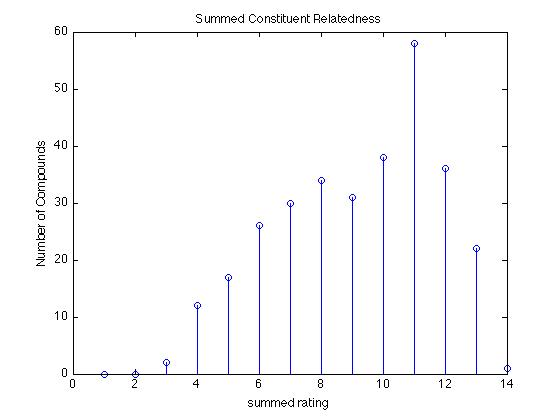
\includegraphics[scale=0.45,bb = 0 0 200 100, draft, type=eps]{/Users/teon/Dropbox/Experiments/NMG/results/stims/compound summed constituent relatedness distribution.jpg}\caption{Distribution of Combined Semantic Relatedness Judgments}
\end{figure}


\end{multicols}

An analysis of naming latencies was conducted for the compounds collected
in the Amazon Mechanical Turk survey using the English Lexicon Project
results \citep{Balota:2007fk}. It suggested a trend toward significance
such that transparent compounds had a shorter latency $[t(\text{130})=-1.77,$
$p=.08]$. As a control, words with no possible internal morphological
construction were added to ensure that the priming effects were not
due to orthography (form priming). These orthographic simple words
were pooled from several studies (see \nameref{Appendix}) with the
restriction that they have a word embedded in them, but they, themselves
are mono-morphemic (e.g. HATCH-hatchet). These orthographics were
selected to have their embedded words have overlapping punctuation
with them (e.g. HATCH-hatchet vs. CORD-cordial). Sixty orthographics
were selected for this study: thirty of them having the embedded words
at the beginning of the word (e.g. HATCH-hatchet) while thirty others
with the embedded words at the end (LOG-dialog). 

In addition, we included novel compounds to look at composition effects
for words with possible morphological structure but with no overall
meaning. Sixty novel compounds were generated using the remaining
compounds from the relatedness survey. The constituents of the novel
compound were randomly selected from the pools of remaining constituents,
respectively. Since these constituents are words that are likely to
be compounded with others, they make good candidates for novel word
formation. To prevent the random formation of an existing word, the
word frequency of these compounds were checked using the English Lexicon
Project's word frequencies \citep{Balota:2007fk}.


\subsection{Experiment Design }

This study contrasted four different word types, each with 60 items:
transparent, opaque, orthographics, and novel compounds. These word
types were compared in two types of priming, repetition and partial
(constituent). For the repetition priming condition, the full compound
was shown as both the prime and the target as compared to the constituent
priming where the constituent of word (in this study, first-constituent
only) is used as a prime for its whole word target. These priming
conditions were compared to their unrelated controls. These conditions
were latin-squared and blocked such that each word appeared in each
of the condition per block. To account for any possible long-lag priming
effects, we factored in block order into our design producing a completely
within-subjects, fully factorial design: Word Type (4) $\times$ Constituency
(2) $\times$ Priming (2) $\times$ Block Order (4). 

\begin{table}[H]
\begin{tabular}{|c||c|c||c|c||c|c||c|c|}
\hline 
\multicolumn{1}{|c|}{\multirow{2}{*}{}} & \multicolumn{2}{c||}{Transparent} & \multicolumn{2}{c||}{Opaque} & \multicolumn{2}{c||}{Novel} & \multicolumn{2}{c|}{Orthographic}\tabularnewline
\cline{2-9} 
 & prime & target & prime & target & prime & target & prime & target\tabularnewline
\hline 
\hline 
control & doorbell & teacup & heirloom & hogwash & keybook & winecloud & brothel & spinach\tabularnewline
\hline 
identity & teacup & teacup & hogwash & hogwash & winecloud & winecloud & spinach & spinach\tabularnewline
\hline 
\hline 
control & door & teacup & heir & hogwash & key & winecloud & broth & spinach\tabularnewline
\hline 
constituent & tea & teacup & hog & hogwash & wine & winecloud & spin & spinach\tabularnewline
\hline 
\end{tabular}

\caption{Design Matrix}
\end{table}
\label{Design Table}


\subsection{Procedure}

Prior to the experiment, each participant was capped with an EasyCap
29-channel passive scalp electrode system placed with electrodes arranged
according to the international 10/20 system. The impedances were measured
and corrected to below 10 k\textgreek{W}. The participant then had
their head shape digitized using the Polhemus Fastrak system. Along
with head shape, five head position marker coils are digitized to
co-register the participant's head inside the MEG helmet where this
coordinate space is later transformed to each participant's MRI space.
The participant was then tested in a magnetically-shielded chamber,
which is integrated with an active shielding system.

The study used a partial priming word naming task. In this task, a
fixation cross first appears followed by a prime then a target. All
of the visual presentations are 300 ms with an inter-stimulus interval
of 600ms. The task is for the participant to read aloud the target
word from the onset on the screen. Audio was sampled from the presentation
of the target to the activation of a voice trigger (see \nameref{Appendix}).
Their production was recorded from the point a voice trigger is activated.
Each participant was presented with 960 trials: 60 words in each of
four word types counterbalanced for each of the four condition.

MEG data were collected using a 157-axial gradiometer MEG system (Kanazawa
Institute of Technology, Nonoichi, Japan) sampling at 1000 Hz with
a low-pass filter at 200 Hz and a notch filter at 60 Hz. Naming latencies
were computed as the time of the target presentation to the activation
of the voice trigger. Voice recordings were recorded for 700 ms after
the activation of the sound trigger to capture the word production.

Blink detection was determined from an SR-Research Eyelink 1000 arm-mounted
eye-tracker. The epochs were baseline corrected using the pre-stimulus
time interval of 200ms. 


\subsection{Participant Recruitment}

Participants were recruited from the New York City community. There
were five right-handed, native English speakers, all having normal
or corrected-to-normal vision. Due to an irrecoverable co-registration
error, only three participants MEG data survived the source estimation.

\begin{figure}[H]
\begin{centering}
\includegraphics[scale=0.1,bb = 0 0 200 100, draft, type=eps]{/Users/teon/Dropbox/Experiments/NMG/results/helmet/R0095_helmet.tif}\includegraphics[scale=0.1,bb = 0 0 200 100, draft, type=eps]{/Users/teon/Dropbox/Experiments/NMG/results/helmet/R0224_helmet.tif}\includegraphics[scale=0.1,bb = 0 0 200 100, draft, type=eps]{/Users/teon/Dropbox/Experiments/NMG/results/helmet/R0498_helmet.tif}\includegraphics[scale=0.1,bb = 0 0 200 100, draft, type=eps]{/Users/teon/Dropbox/Experiments/NMG/results/helmet/R0499_helmet.tif}\includegraphics[scale=0.1,bb = 0 0 200 100, draft, type=eps]{/Users/teon/Dropbox/Experiments/NMG/results/helmet/R0504_helmet.tif}
\par\end{centering}

\caption{MEG Subject Head Placement}
\end{figure}



\subsection{Analysis}

For behavioral results, the effects on naming latency from the participants'
word production were analyzed using a repeated-measures ANOVA. Naming
latencies were defined as the duration from the visual onset of the
target stimulus to the activation of the voice trigger marked by a
sound threshold. 

For the MEG brain responses, the MEG signal was recorded using a DC
recording with a low-pass filter of 200Hz and a notch filter of 60Hz.
During on-line recording, three axial gradiometers measured the magnetic
fields away from the participant's head but within the dewar. The
brain response MEG signal was then processed using a continuously
adjusted least squares method (CALM) based on these gradiometers to
reduce lower frequency noise from the environment \citep{Adachi:2001wl}.
Lastly, the signal then has a low-pass filter applied at 30Hz.For
both the MEG and EEG brain responses, the data were epoched with a
baseline of 200ms prior to the onset of the target stimulus to 400ms
for MEG and to 500ms for EEG post-stimulus presentation. Trials were
rejected using the Eyelink blink detection. Additionally, MEG trials
were rejected if the signal's amplitude exceeded a threshold of 3pT
throughout the epoch. Since our analyses were interested in the local
brain activity of these regions of interests: fusiform gyrus, temporal
pole, superior temporal gyrus, pars triangularis, and orbitofrontal
cortex, we conducted a cortically-constrained L2 minimum-norm current
estimate using the software package, MNE (Martinos Center for Biomedical
Imaging). Due to an existing noise problem that has been characterized
with a particular topography across a score of participants, a principal
component analysis was conducted to remove this component from the
data.

\begin{figure}[H]
\begin{centering}
\includegraphics[scale=0.1,bb = 0 0 200 100, draft, type=eps]{/Users/teon/Dropbox/Experiments/NMG/results/pca/R0095_pca.png}\includegraphics[scale=0.1,bb = 0 0 200 100, draft, type=eps]{/Users/teon/Dropbox/Experiments/NMG/results/pca/R0224_pca.png}\includegraphics[scale=0.1,bb = 0 0 200 100, draft, type=eps]{/Users/teon/Dropbox/Experiments/NMG/results/pca/R0498_pca.png}\includegraphics[scale=0.1,bb = 0 0 200 100, draft, type=eps]{/Users/teon/Dropbox/Experiments/NMG/results/pca/R0499_pca.png}\includegraphics[scale=0.1,bb = 0 0 200 100, draft, type=eps]{/Users/teon/Dropbox/Experiments/NMG/results/pca/R0504_pca.png}
\par\end{centering}

\caption{PCA across subjects}
\end{figure}


A noise covariance matrix was computed to correlate sensors with each
other in the presence of ambient noise. To prevent correlating ambient
noise and brain response, we used a 400 ms epoch window centered on
the presentation of the fixation cross. This allows for the computation
on recorded data that is individually tuned. The sensor locations
are then transformed into MRI space to have these sources in a common
space. Using the covariance matrix, the MEG sensor coordinate transformation,
and the MRI, a forward model is computed to estimate the how cortical
source activity would be realized at an MEG sensor. Our MRIs are parcellated
into 5124 icosahedron sources. Since this forward model is generally
well-understood, we can generate an inverse operator and apply it
to the MEG data to solve the sensor-to-source problem. Our event-related
fields (ERFs) were defined based on the previous work and are generally
accepted time windows: 100-200ms (M170), 200-300ms (M250), 300-400ms
(M350), all post-stimulus presentation \citep{Pylkkanen:2003fk}.

\begin{multicols}{2}The EEG data was analyzed using a cluster-based
sensor approach \citep{Morris:2007uq}. Since our electrode cap differed
slightly from prior work, we adjusted the clusters to reflect comparable
areas. Electrodes were classified into four clusters: outer (Fp1,
Fp2, O1, O2, F7, F8, P7, P8), midlateral (F3, F4, P3, P4, FC5, FC6,
CP5, CP6), inner (C3, C4, FC1, FC2, CP1, CP2), and midline (Fz, FCz,
Cz, CPz, Pz, POz).

\begin{figure}[H]
\begin{centering}
\includegraphics[scale=0.67,bb = 0 0 200 100, draft, type=eps]{/Users/teon/Dropbox/Experiments/NMG/results/rois/cap arrangement.png}
\par\end{centering}

\caption{EEG Electrode Arrangement}
\end{figure}


\end{multicols}

There were two windows of interests for the event-related potentials
(ERPs) in this study: 200-300ms (N250) and the 300-500ms (N400), all
post-stimulus presentation.


\section{Results}


\subsection{Behavioral}

\begin{multicols}{2}For the behavioral results, in the repetition
priming condition, latency analyses revealed that there is a significant
effect in priming such that naming latencies were shorter for the
target when it was primed $[F_{1}(1,4)=47.64,$ $p=.00]$. There was
also an significant effect of word type $[F_{1}(3,4)=4.12,$ $p=.03]$
and block order $[F_{1}(3,4)=7.71,$ $p=.05]$. There was no significant
interaction between word type and priming $[F_{1}(1,4)=2.38,$ $p=.12]$

\begin{figure}[H]
\begin{centering}
\includegraphics[scale=0.4,bb = 0 0 200 100, draft, type=eps]{/Users/teon/Dropbox/Experiments/NMG/results/plots/behavioral/latency_identity.png}
\par\end{centering}

\caption{Repetition Priming on Naming Latency}
\end{figure}


\end{multicols}

\begin{multicols}{2}

\begin{figure}[H]
\begin{centering}
\includegraphics[scale=0.4,bb = 0 0 200 100, draft, type=eps]{/Users/teon/Dropbox/Experiments/NMG/results/plots/behavioral/latency_constituent.png}
\par\end{centering}

\caption{Partial Priming on Naming Latency}
\end{figure}


For the partial priming condition, analyses revealed that there is
a significant effect in priming such that naming latencies were shorter
for the target when it was primed $[F_{1}(1,4)=11.87,$ $p=.02]$.
There was also an significant effect of block order $[F_{1}(1,4)=10.20,$
$p=.03]$, but there was only a trend toward an interaction effect
of word type and priming $[F_{1}(1,4)=2.83,$ $p=.08]$ such that
naming latency are faster for transparent, opaque and novel compounds
but not for the orthographic simple words. 

\end{multicols}


\subsection{MEG}

Due to the anomalous co-registration error, non-removable environmental
noise, and the sparse participant sample, there is not enough statistical
power to reliably test our predictions. However, we can observe the
trends in the data for our regions of interest. Below, repetition
priming is referred to as RP and partial priming, PP.


\subsubsection{\noindent Left Fusiform Gyrus}

There appears to be a trend of decreased activation in the repetition
condition beginning in the M170 window expanding to the M250.

\begin{multicols}{2}

\begin{figure}[H]
\begin{centering}
\includegraphics[scale=0.4,bb = 0 0 200 100, draft, type=eps]{/Users/teon/Dropbox/Experiments/NMG/results/plots/meg/erfs/priming_lh.fusiform_identity.png}
\par\end{centering}

\caption{Grand Averages of RP Activation}


\caption{M170 RP Activation per Word Type }
\end{figure}
\columnbreak

\begin{figure}[H]
\includegraphics[height=2in,bb = 0 0 200 100, draft, type=eps]{/Users/teon/Dropbox/Experiments/NMG/results/plots/meg/bars/fusiform-identity_m170.png}
\end{figure}


\end{multicols}

\noindent Here, there is an interaction pattern in the partial priming
condition between word type and priming. Novel and opaque compounds
pattern together with more activation in the primed condition whilst
transparent compounds show a decrease in activation.

\begin{multicols}{2}

\begin{figure}[H]
\begin{centering}
\includegraphics[scale=0.4,bb = 0 0 200 100, draft, type=eps]{/Users/teon/Dropbox/Experiments/NMG/results/plots/meg/erfs/priming_lh.fusiform_constituent.png}
\par\end{centering}

\caption{Grand Averages of PP Activation}


\caption{M170 PP Activation per Word Type }
\end{figure}
\columnbreak

\begin{figure}[H]
\includegraphics[height=2in,bb = 0 0 200 100, draft, type=eps]{/Users/teon/Dropbox/Experiments/NMG/results/plots/meg/bars/fusiform-constituent_m170.png}
\end{figure}


\end{multicols}


\subsubsection{\noindent Temporal Pole}

There appears to be a trend of decreased activation in the repetition
condition peaking around the M250 window.

\begin{multicols}{2}

\begin{figure}[H]
\begin{centering}
\includegraphics[scale=0.4,bb = 0 0 200 100, draft, type=eps]{/Users/teon/Dropbox/Experiments/NMG/results/plots/meg/erfs/priming_lh.temporalpole_identity.png}
\par\end{centering}

\caption{Grand Averages of RP Activation}


\caption{M250 RP Activation per Word Type }
\end{figure}
\columnbreak

\begin{figure}[H]
\includegraphics[height=2in,bb = 0 0 200 100, draft, type=eps]{/Users/teon/Dropbox/Experiments/NMG/results/plots/meg/bars/temporalpole-identity_m250.png}
\end{figure}


\end{multicols}

Here, there is an interaction pattern in the partial priming condition
between word type and priming. Novel and opaque compounds pattern
together with more activation in the primed condition.

\begin{multicols}{2}

\begin{figure}[H]
\begin{centering}
\includegraphics[scale=0.4,bb = 0 0 200 100, draft, type=eps]{/Users/teon/Dropbox/Experiments/NMG/results/plots/meg/erfs/priming_lh.temporalpole_constituent.png}
\par\end{centering}

\caption{Grand Averages of PP Activation}


\caption{M250 PP Activation per Word Type }
\end{figure}
\columnbreak

\begin{figure}[H]
\includegraphics[height=2in,bb = 0 0 200 100, draft, type=eps]{/Users/teon/Dropbox/Experiments/NMG/results/plots/meg/bars/temporalpole-constituent_m250.png}
\end{figure}


\end{multicols}


\subsubsection{\noindent Orbitofrontal Cortex}

There appears to be a trend of decreased activation in the repetition
condition beginning around 200ms within the M250 window. 

\begin{multicols}{2}

\begin{figure}[H]
\begin{centering}
\includegraphics[scale=0.4,bb = 0 0 200 100, draft, type=eps]{/Users/teon/Dropbox/Experiments/NMG/results/plots/meg/erfs/priming_lh.medialorbitofrontal_identity.png}
\par\end{centering}

\caption{Grand Averages of RP Activation}


\caption{M250 RP Activation per Word Type }
\end{figure}
\columnbreak

\begin{figure}[H]
\includegraphics[height=2in,bb = 0 0 200 100, draft, type=eps]{/Users/teon/Dropbox/Experiments/NMG/results/plots/meg/bars/medialorbitofrontal-identity_m250.png}
\end{figure}


\end{multicols}

Here, there is an interaction pattern in the partial priming condition
between word type and priming. Opaque compounds show more activation
in the primed condition than any word type. Transparent compounds
have the opposite pattern of activation showing a decrease in activation
when primed.

\begin{multicols}{2}

\begin{figure}[H]
\begin{centering}
\includegraphics[scale=0.4,bb = 0 0 200 100, draft, type=eps]{/Users/teon/Dropbox/Experiments/NMG/results/plots/meg/erfs/priming_lh.medialorbitofrontal_constituent.png}
\par\end{centering}

\caption{Grand Averages of PP Activation}


\caption{M250 PP Activation per Word Type }
\end{figure}
\columnbreak

\begin{figure}[H]
\includegraphics[height=2in,bb = 0 0 200 100, draft, type=eps]{/Users/teon/Dropbox/Experiments/NMG/results/plots/meg/bars/medialorbitofrontal-constituent_m250.png}
\end{figure}


\end{multicols}


\subsubsection{\noindent Superior Temporal Gyrus}

There appears to be a trend of an interaction in the repetition condition
where transparent compounds exhibit decreased activation the M250
window.

\begin{multicols}{2}

\begin{figure}[H]
\begin{centering}
\includegraphics[scale=0.4,bb = 0 0 200 100, draft, type=eps]{/Users/teon/Dropbox/Experiments/NMG/results/plots/meg/erfs/priming_lh.superiortemporal_identity.png}
\par\end{centering}

\caption{Grand Averages of RP Activation}


\caption{M250 RP Activation per Word Type }
\end{figure}
\columnbreak

\begin{figure}[H]
\includegraphics[height=2in,bb = 0 0 200 100, draft, type=eps]{/Users/teon/Dropbox/Experiments/NMG/results/plots/meg/bars/superiortemporal-identity_m250.png}
\end{figure}


\end{multicols}

Here in the partial priming condition, opaque compounds pattern show
a increase of activation in the primed condition.

\begin{multicols}{2}

\begin{figure}[H]
\begin{centering}
\includegraphics[scale=0.4,bb = 0 0 200 100, draft, type=eps]{/Users/teon/Dropbox/Experiments/NMG/results/plots/meg/erfs/priming_lh.temporalpole_constituent.png}
\par\end{centering}

\caption{Grand Averages of PP Activation}


\caption{M250 PP Activation per Word Type }
\end{figure}
\columnbreak

\begin{figure}[H]
\includegraphics[height=2in,bb = 0 0 200 100, draft, type=eps]{/Users/teon/Dropbox/Experiments/NMG/results/plots/meg/bars/superiortemporal-constituent_m250.png}
\end{figure}


\end{multicols}


\subsubsection{\noindent Pars Triangularis}

\noindent In the repetition condition, there appears to be a sustained
deactivation beginning around the M170 window while overlapping the
M250. Transparent compounds tend to have the strong effect from this
repetition.

\begin{multicols}{2}

\begin{figure}[H]
\begin{centering}
\includegraphics[scale=0.4,bb = 0 0 200 100, draft, type=eps]{/Users/teon/Dropbox/Experiments/NMG/results/plots/meg/erfs/priming_lh.parstriangularis_identity.png}
\par\end{centering}

\caption{Grand Averages of RP Activation}


\caption{M250 RP Activation per Word Type }
\end{figure}
\columnbreak

\begin{figure}[H]
\includegraphics[height=2in,bb = 0 0 200 100, draft, type=eps]{/Users/teon/Dropbox/Experiments/NMG/results/plots/meg/bars/parstriangularis-identity_m250.png}
\end{figure}


\end{multicols}

Here, there is an interaction pattern in the partial priming condition
between word type and priming. Novel and opaque compounds have again
patterned together with more activation in the primed condition. There
appears to be less activation for the transparent compounds when primed
and nearly no effect on the orthographic simple words.

\begin{multicols}{2}

\begin{figure}[H]
\begin{centering}
\includegraphics[scale=0.4,bb = 0 0 200 100, draft, type=eps]{/Users/teon/Dropbox/Experiments/NMG/results/plots/meg/erfs/priming_lh.parstriangularis_constituent.png}
\par\end{centering}

\caption{Grand Averages of PP Activation}


\caption{M250 PP Activation per Word Type }
\end{figure}
\columnbreak

\begin{figure}[H]
\includegraphics[height=2in,bb = 0 0 200 100, draft, type=eps]{/Users/teon/Dropbox/Experiments/NMG/results/plots/meg/bars/parstriangularis-constituent_m250.png}
\end{figure}


\end{multicols}


\subsection{EEG}

Analyses revealed a pattern of surprising results. The task yielded
a component that was centered between the two time regions of interests,
N250 and N400. This component appears to be a P300 with opposite field
pattern polarity than was expected. The priming manipulation yields
strong amplitude modulations irrespective of word type. Thus, the
following analyses will investigate the P300 effects.


\subsubsection{Outer cluster}

\begin{multicols}{2}

Analyses for repetition priming condition revealed a significant priming
effect, $[F_{1}(1,4)=16.20,$ $p=.03]$. No other effect was significant.

\begin{figure}[H]
\centering{}\includegraphics[scale=0.4,bb = 0 0 200 100, draft, type=eps]{/Users/teon/Dropbox/Experiments/NMG/results/plots/eeg/erps/priming_outer_identity.png}
\end{figure}


\end{multicols}

\begin{multicols}{2}

A significant priming was also found for the partial priming condition,
$[F_{1}(1,4)=122.36,$ $p=.00]$. No other effect was significant.

\begin{figure}[H]
\centering{}\includegraphics[scale=0.4,bb = 0 0 200 100, draft, type=eps]{/Users/teon/Dropbox/Experiments/NMG/results/plots/eeg/erps/priming_outer_constituent.png}
\end{figure}


\end{multicols}


\subsubsection{Midlateral cluster}

\begin{multicols}{2}

\begin{figure}[H]
\centering{}\includegraphics[scale=0.4,bb = 0 0 200 100, draft, type=eps]{/Users/teon/Dropbox/Experiments/NMG/results/plots/eeg/erps/priming_midlateral_identity.png}
\end{figure}


Analyses for repetition priming condition revealed a significant priming
effect, $[F_{1}(1,4)=14.37,$ $p=.03]$.

\end{multicols}

\begin{multicols}{2}

\begin{figure}[H]
\centering{}\includegraphics[scale=0.4,bb = 0 0 200 100, draft, type=eps]{/Users/teon/Dropbox/Experiments/NMG/results/plots/eeg/erps/priming_midlateral_constituent.png}
\end{figure}


A significant priming was also found for the partial priming condition,
$[F_{1}(1,4)=55.15,$ $p=.01]$. No other effect was significant.

\end{multicols}


\subsubsection{Inner cluster}

\begin{multicols}{2}

Analyses for repetition priming condition revealed a significant priming
effect, $[F_{1}(1,4)=16.72,$ $p=.03]$. 

\begin{figure}[H]
\centering{}\includegraphics[scale=0.4,bb = 0 0 200 100, draft, type=eps]{/Users/teon/Dropbox/Experiments/NMG/results/plots/eeg/erps/priming_inner_identity.png}
\end{figure}


\end{multicols}

\begin{multicols}{2}

A significant priming was also found for the partial priming condition,
$[F_{1}(1,4)=40.21,$ $p=.01]$. No other effect was significant.

\begin{figure}[H]
\centering{}\includegraphics[scale=0.4,bb = 0 0 200 100, draft, type=eps]{/Users/teon/Dropbox/Experiments/NMG/results/plots/eeg/erps/priming_inner_constituent.png}
\end{figure}


\end{multicols}


\subsubsection{Midline cluster}

\begin{multicols}{2}

\begin{figure}[H]
\centering{}\includegraphics[scale=0.4,bb = 0 0 200 100, draft, type=eps]{/Users/teon/Dropbox/Experiments/NMG/results/plots/eeg/erps/priming_midline_identity.png}
\end{figure}


Analyses for repetition priming condition revealed a significant priming
effect, $[F_{1}(1,4)=18.96,$ $p=.02]$. In addition, a borderline
significant condition by block order interaction was found, $[F_{1}(1,4)=3.88,$
$p=.05]$. 

\end{multicols}

\begin{multicols}{2}

\begin{figure}[H]
\centering{}\includegraphics[scale=0.4,bb = 0 0 200 100, draft, type=eps]{/Users/teon/Dropbox/Experiments/NMG/results/plots/eeg/erps/priming_midline_constituent.png}
\end{figure}


A significant priming was also found for the partial priming condition,
$[F_{1}(1,4)=35.68,$ $p=.01]$. No other effect was significant.

\end{multicols}


\section{Discussion}


\subsection{Behavioral}

The word naming latency effect is largely consistent with the masked
priming literature on word recognition demonstrating the interaction
where complex words pattern together having a reduced latency due
to priming while priming simple words do not any effects on latency
due to priming \citep{McCormick:2008mn,Morris:2007uq,Rastle:2004bh,Taft:2004uq}.
However, these priming effects are not consistent with the effects
demonstrated in the semantic priming literature. Here, there is an
interaction among the complex words such that transparent complex
words have a faster reaction time but opaque complex words have a
lower reaction time compared to baseline \citep{Rastle:2000xo}. This
effect is rather surprising because it suggests that there is no effect
of semantic transparency on naming latency. This effect also departs
from the predicted pattern from the English Lexicon Project analysis
where there was a difference in the naming latency for transparent
and opaque compounds. Naming latency effects may not be sensitive
enough to reveal any semantic transparency difference. Because the
naming latency effects pattern with the lexical decision effects in
previous work, this suggests that morphological decomposition has
occurred in the recognition process. That is, complex words do show
this automatic segmentation, which is consistent with the proposed
morphological composition model of word recognition.


\subsection{MEG}

The MEG results on repetition priming showed some patterns consistent
with the predictions for the fusiform gyrus: there was decreased activity
for across all word types when a word was repeated, which is a consistent
finding \citep{Fiebach:2005fk}. For partial priming, there was a
pattern of an interaction where opaque compounds had more cortically
activation than transparent which showed reduced activation. This
semantic transparency effect may be attributable to SOA where prolonged
conscious awareness may cause the increased brain activity of opaque
compounds since the meaning of its prime is incongruous with its meaning.

For the temporal pole, pars triangularis, superior temporal gyrus,
and orbitofrontal cortex, there was a pattern of an interaction such
that primed opaque compounds lead to more activity. All areas but
the superior temporal gyrus showed patterns of decreased activity
for transparent compounds when they were primed. The effects in these
regions correspond in time and in location to previously defined regions
of composition \citep{Bemis:2011zr,Pylkkanen:2007yq}. These patterns
are consistent with the composition model where meaning integration
has different effects across the dimensions of semantic transparency.
That is, transparent compounds have decreased activity when primed,
which is consistent with semantic priming studies \citep{Matsumoto:2005lw}.
However, opaque compounds have increased activation when primed. These
results fit in with the morphological composition model where there
would be a decrease in activation if there is a semantic relationship
between the prime and target.


\subsection{EEG}

The EEG results revealed an unexpected component that strongly signaled
an effect with priming. The P300 component has been associated with
anticipation of an infrequent but expected stimulus \citep{Verleger:1994ys}.
Since our task operated on overt semantic priming where our stimulus-onset
asynchrony is 600ms, it may have led participant to anticipate our
prime trials more than a more subtle, covert prime. The choice of
SOA came from composition studies where priming was not used, leading
the composition to be less obvious \citep{Bemis:2011zr}, but given
the task, a faster SOA may be more appropriate. Studies investigating
differential semantic processes during word recognition have used
times half as long as the ones in composition studies \citep{Rastle:2000hg}.
The current SOA may also be problematic because it has a prolonged
conscious representation, which may confound the subprocesses typically
associated with word recognition. This would perhaps decrease the
possibility of strategic behavior. This P300 effect may have shrouded
the ERP components of interests since its time window overlaps both
the N250 and the N400 windows.


\subsection*{Conclusions}

There appears to be evidence that there are stages of processing in
visual word recognition that reflects morphological-based parsing
and computation. The behavioral effects from word naming demonstrate
a pattern of results consistent with the existing literature on the
early stages of visual word recognition. Source estimates over the
time-course of recognition revealed key patterns of activation consistent
with predictions from a morphological composition-based theory of
word recognition. Activation in the fusiform reflect automatic segmentation
in morphologically complex words that leads to lexical access. These
processes are followed by a stage of composition where constituents
of a word are recombined in a ``lock-and-key'' fashion to construct
the meaning of the overall word. This study informs our understanding
of what information is stored in the mental lexicon. Word forms are
the lexical entry of choice for providing the meaning and the instruction
for constructing more complex words. The combination of these word
forms yields new meaning from the basis of established ones. This
consistency of composition across different levels of processing:
phrase-level \citep{Bemis:2011zr} and word-level, may provide insight
to whether there is a general binding principle that governs all levels
of language construction.

Critically, a new SOA would be the most informative of the semantic
nature of morphological composition. Evidence from behavioral studies
point to a shorter SOA than our current study as it ``allows conscious
appreciation of the primes, yet may be so brief as to minimise strategic
behaviour'' \citep{Rastle:2000xo}. An increase of participants would
yield enough power to effectively evaluation the significance of the
pattern of results. The concurrent measures of EEG and MEG provided
equally informative and different sources of information. 

Since this dataset provides a rich source of information regarding
word processing, an analysis of acoustic duration will inform our
notion of lexical integrity. Evidence in the word production literature
suggests that giveness, the relative activation of an item, of a discourse
entity may lead to acoustic reduction in their pronunciation \citep{Kahn:2012io}.
Since priming leads to an activation effect in word recognition, partial
priming of the constituent should lead to facilitation of the phonological
code of that constituent within its compound. If this holds true,
there should be an acoustic reduction for compounds when partially
primed but no reduction for orthographics. This would add more evidence
that discounts the lexical integrity hypothesis assumption that words
are a solitary and indivisible unit \citep{Lapointe:1980xk}. These
analyses will broaden our understanding of the architecture of the
mental lexicon and how composition integrates word forms and gives
rise to new meaning.


\section{Appendix\label{Appendix}}

The compounds were pooled from \citet{Drieghe:2010vn,Fiorentino:2007kw,Fiorentino:2009:xi,Juhasz:2003ka}.
The semantic relatedness norming procedure was replicated over the
pooled list of compounds. The ratings were largely consistent with
the prior work. The orthographic simple words were pooled from \citet{Rastle:2004bh}
and \citet{Balota:2007fk}.

Psychtoolbox monitors the audio throughout the recording session.
Latency times are measured from the presentation of the target screen
to onset of the voice trigger: when the acoustic noise exceeds the
set threshold (0.1), it sends a trigger to the MEG, the EEG and presentation
computer to mark the beginning of speech and naming latency times.

\bibliographystyle{apalike2}
\bibliography{/Users/teon/Dropbox/articles/library}

\end{document}
